\documentclass[draft,linenumbers]{agujournal}

\draftfalse

\usepackage{hyperref}
\hypersetup{
colorlinks=true,
linkcolor=blue,
filecolor=magenta,
urlcolor=cyan}

\journalname{Journal of Advances in Modeling Earth Systems (JAMES)}

\begin{document}
%tentative author list...
\authors{Rosie A. Fisher\affil{1},
William Wieder\affil{1,2},
Benjamin M. Sanderson\affil{3},
Charles D. Koven\affil{4},
Keith W. Oleson\affil{1},
Chonggang Xu\affil{5},
Joshua Fisher\aff B.il{6},
Mingjie Shi\affil{6},
Anthony P. Walker\affil{7},
Gordon B. Bonan\affil{1},
David M. Lawrence\affil{1}
}

\title{Parameteric controls on responses to biogeochemical forcing in the CLM5}
\author{Rosie Fisher}
\date{November 2018}

\affiliation{1}{National Center for Atmospheric Research, Table Mesa Drive, Boulder, Colorado, USA}

\affiliation{2}{Institute of Arctic and Alpine Research, University of Colorado, Boulder Colorado, USA}

\affiliation{3}{Centre Europe'en Research et de Formation Avenc'ee en Calcul Scientifique, Toulouse, France}

\affiliation{4}{Lawrence Berkeley National Laboratory, Berkeley, California, USA}

\affiliation{5}{Los Alamos National Laboratory, Los Alamos, New Mexico, USA}

\affiliation{6}{NASA Jet Propulsion Laboratory, Pasadena, California, USA}

\affiliation{7}{Oak Ridge National Laboratory, Oak Ridge, Tennessee, USA}

\correspondingauthor{Rosie Fisher}{rfisher@ucar.edu}


\begin{keypoints}
\item The Community Land Model, version 5, contains numerous upgrades to carbon and nitrogen cycling.

\item Model state and responses to CO$_{2}$ and nitrogen addition are sensitive to parameter choice.

\item Parameters controlling nitrogen fixation, uptake, and stoichiometric flexibilty are most important
\end{keypoints}

\begin{abstract}
A suite of modifications to the nitrogen cycle representation were added to the Community Land Model, version 5.  New features of the model include prognostic $V_{c,max}$ and $J_{max}$, representation of the carbon economic cost of nitrogen uptake, switching of N uptake between alternative sources, variable tissue C:N ratios and dynamic leaf resorption of nitrogen.

Here we assess the sensitivity of the model to a suite of parameters pertinent to the cycling of carbon and nitrogen. We assess the dependence of both the model state, and also the responses of the system to CO$_{2}$ and nitrogen fertilization to parametric uncertainty. Model runs are conducted at representative individual sites in temperate, tropical and boreal systems.

The model responses to CO$_{2}$  and N fertilization are primarily linked to the representation of the fraction of plants that can fix nitrogen, the costs of N in the environment and stoichiometric flexibility of plant tissues, all of which are subject to large empirical and theoretical uncertainty.  Identification of the primary factors driving ecosystem responses to fertilization assists in the interpretation of global simulations and in the identification of priorities for fieldwork and process updates.
\end{abstract}

\section{Introduction}
Simulating the cycling of nutrients, and how nutrient availability impacts ecosystem growth and function, has been repeatedly identified as a crucial element of Earth system models (\cite{piao2013}, \cite{gruber2008}, \cite{wang2009}). In the CMIP5 multi-model inter-comparison, only one land model, the Community Land Model v4 (CLM4), included an active nitrogen (N) cycle. The CLM4 projected that inclusion of N dynamics might significantly limit the ability of the terrestrial biosphere to respond to fertilization by increasing atmospheric carbon dioxide ( \cite{friedlingstein2006}, \cite{thornton2007} \cite{friedlingstein2014}, \cite{arora2013}). Subsequent and parallel to CMIP5, many terrestrial biosphere and land surface models that represent global N dynamics using alternative structural assumptions have been developed (\cite{wang2007}, \cite{zaehle2010}, \cite{goll2012}, \cite{smith2014}). Nonetheless, substantial uncertainty remains in the land surface modeling community regarding how nutrient limitations should be represented in models (\cite{zaehledalmonech2011}).

Unlike representations of photosynthetic responses to environmental conditions, or radiative transfer through forest canopies, our understanding of how nutrient cycling functions both within plants and in whole ecosystems is not governed by any well-tested and widely accepted paradigms. Detailed model-data synthesis activities, notably those conducted at North American free-air carbon dioxide enrichment (FACE) experiments, have revealed important differences in model behavior emerging in part from the absence of a broadly accepted theoretical framework for construction and parameterization of nutrient cycling processes (\cite{kauwe2013}, \cite{zaehle2014}, \cite{medlyn2015}). Few studies, however, have looked at how CO$_{2}$ or N fertilization are governed by the parameters or structure of a given model (c.f. \cite{meyerholt2018}).

The Community Land Model is the land surface representation within the Community Earth System Model (CESM, \cite{hurrell2013}). Version 5 of the CLM was released to the research community as part of the CESM2.0 release and open-source releases and development are housed at \url{https://github.com/ESCOMP/ctsm/}. An overview of model developments is presented by \cite{lawrence2018}, a description of the global nitrogen cycling by Wieder et al. (2018), the crop model by(Lombardozzi et al. in prep), the land use components by (Lawrence P et al. in prep), and plant hydraulics by (Kennedy et al., 2018).

CLM5 includes numerous major updates of the nitrogen cycle representation relative to CLM4 and CLM4.5 (\cite{lawrence2011}). The introduction of several new dynamical features into the CLM5 has implications for both parametric uncertainty and responses to environmental forcing. Wieder et al. (2018) report the global-scale carbon cycle implications of the full model update and note that, in CLM5, carbon uptake responds more strongly to CO$_{2}$ and less strongly to N fertilization than its predecessors.  In this paper, we describe the new components of the biogeochemical cycling, and investigate the features of the new model that control the model state and biogeochemical forcing responses in depth, using single-site experiments and parametric sensitivity analyses. 

\subsection{Model Updates}
The CLM5 nitrogen cycle builds on the implementation of carbon-nitrogen interactions in the CLM4 model (\cite{thornton2007}), and on modifications to the biogeochemical cycling (notably vertically stratified soil decomposition processes) included in the CLM4.5 (\cite{koven2013}, \cite{bonan2012}). The new model integrates three major additional prognostic elements of the nitrogen cycle, including:\\

1) The `LUNA' module (Leaf Utilization of Nitrogen for Assimilation), which simulates distribution of N between different leaf assimilation processes (\cite{xu2012}, \cite{ali2016}) \\

2) The `FUN' module (Fixation and Uptake of Nitrogen), which simulates the dynamics and carbon economics of N acquisition from the environment (\cite{fisher2010fun}, \cite{brzostek2014}, \cite{shi2016}), and\\

3) The `FLEXCN' N cycle implementation, adapted from \cite{ghimire2016}, which is used in CLM5 primarily to allow variation in tissue C:N ratios.\\

More details on each of these new components is given below. A full technical description of the CLM5 is an appendix to \cite{lawrence2018} and is also available online at \url{(https://escomp.github.io/ctsm-docs/doc/build/html/tech_note/index.html).}

\subsubsection{LUNA}
Most land surface models predict photosynthetic parameters from leaf nitrogen content (\cite{kattge2009}, \cite{bonan2012}). There is significant evidence, however, that plant photosynthetic capacity can respond to environmental conditions, including CO$_{2}$ fertilization (\cite{ainsworth2007}) and changing temperature (\cite{hikosaka2005}), irradiance (\cite{niinemets1998}) and soil moisture (\cite{keenan2009}). Given the importance of photosynthetic capacity as a key model parameter (\cite{rogers2017}) the use of a static photosynthetic capacity appears to be a poor means of capturing its variation in time and space and responses to climatic change (\cite{walker2017}).

Given a specific amount of leaf N and empirical environmental constraints, the LUNA model predicts the optimal partitioning of N among the maximum rate of carboxylation $V_{c,max}$, the maximum rate of electron transport $J_{max}$, and other leaf N components, for the prevailing time-averaged environmental conditions. The model determines the rate constants that are consistent with a co-limitation of photosynthesis by both electron capture and carboxylation processes. In this fashion, $V_{c,max}$ is primarily controlled by the N per unit leaf area $N_{area}$, (which is itself a function of the target C/N ratio, the specific leaf area, and the prognostic variation in leaf C/N ratios) and prevailing environmental conditions (CO$_{2}$, temperature, humidity, soil moisture, radiation and day length). The capacity of the LUNA model to represent appropriate responses to temperature and CO$_{2}$ was assessed by \cite{xu2012} while the improved codes for global calibration and the geographical predictions of the model were described by \cite{ali2016}. 

\subsubsection{FUN}
Under circumstances where insufficient N uptake was available to match all of the carbon assimilated (for a given target C:N ratio), the CLM4 model reduced the gross photosynthetic flux down to the level at which growth could be supported by N uptake. This process occurred after the calculation of stomatal conductance (which is linked to assimilation rates via the Ball-Berry model) and therefore created inconsistencies between C assimilation and water cycling, especially under conditions of N limitation, as discussed extensively in the literature (\cite{medlyn2011}, \cite{bonan2012}, \cite{dekauwe2014}, \cite{walker2014}).

One major issue confronting N cycle models is how to deal with this 'excess' carbon under N limiting conditions (\cite{zaehle2010}, \cite{dekauwe2014}). The FUN model (\cite{fisher2010fun}, \cite{brzostek2014}, \cite{shi2016}) addresses this issue by imposing the principle that for the alternative sources of nitrogen acquisition by plants (active uptake from soil, retranslocation from senescent tissues, and symbiotic N fixation) there is a concurrent cost in terms of carbon (\cite{bloom1985}, \cite{jiang2017}, \cite{terrer2018}). Further, the cost of each uptake pathway is variable in both time and space. FUN hypothesizes that plants will take up nitrogen from pathways which are 'cheaper' to them. Where N is scarce in the environment, carbon that would otherwise have been used for plant growth (net primary productivity, NPP) can be deployed to acquire (pay for) more N. Thus, N limitation leads to reduced growth and higher expenditure of C on N uptake (and reduces carbon use efficiency- defined here as NPP divided by gross primary productivity, GPP). The central element of FUN is a set of simultaneous equations which assume, firstly, that the total carbon available (after maintenance respiration and replenishment of stores are accounted for), `$C_{avail}$', is either used for plant growth ($C_{growth}$) or for nitrogen uptake, ($C_{nuptake}$).

\begin{equation}
C_{growth}=C_{avail}-C_{nuptake}
\end{equation}

Further, the nitrogen acquired from the environment ($N_{uptake}$) must equal the amount spent on N divided by it's average cost ($N_{cost}$), and also the amount of carbon deployed for growth divided by the plant C:N ratio ($CN_{plant}$):

\begin{equation}
N_{uptake}=C_{nuptake}/N_{cost} =\frac{C_{growth}}{(CN_{plant}/(1.0+f_{gr})}
\end{equation}

The carbon used for growth is further reduced by the growth respiration term ($f_{gr}$, which applies only to tissues that are constructed). Rearrangement of these constraints gives a predictive term for the amount of carbon that is expended on N uptake, as:

\begin{equation}
C_{nuptake} =\frac{C_{avail}}{ ( (1.0+f_{gr})*(CN_{plant} / N_{cost}) + 1) }
\end{equation}

The average nitrogen cost ($N_{cost}$) is derived from the uptake of N, weighted for its cost across all uptake streams, while the plant CN ratio ($CN_{plant}$) is the combined target CN ratio of all the plant tissues, weighted for the size of the different pools. The FUN model is documented at \url{https://escomp.github.io/ctsm-docs/doc/build/html/tech_note/FUN/CLM50_Tech_Note_FUN.html}

One mechanism introduced by FUN is the preferential use of symbiotic N fixation when soil mineral N concentrations are low (\cite{vitousek2002}). The CLM4 and CLM4.5 predict N fixation as a linear function of net primary productivity (\cite{cleveland1999}), and \cite{wieder2015} illustrated the impacts of uncertainty in this function.  FUN considers fixation rates to be an emergent property of plant assimilation rates, the relative costs of environmental N acquisition compared to fixation, and temperature (which exerts a primary control over the enzymatic processes, following \cite{houlton2008}). Fixation is preferred when the costs of `active' N acquisition from soil are higher than that of fixation. 

Note that while the CLM5 has no representation of biological succession (\cite{fisher2018}), this property nonetheless affects the amount of time taken to achieve a spun-up state (carbon and nitrogen pools in equilibrium) from bare ground. In most cases, N fixation is preferred when soil N is low, and so soil N builds up quickly. In low productivity areas, however, carbon is required to fix N from a 'cold start' initial state, impacting the carbon use efficiency and survival of marginal plants; thus higher initial stocks of N are required to allow growth once metabolic and turnover costs have been met in early spin-up.

The FUN model introduces the concept of carbon payments for N uptake, which are analagous to the carbon expended on root exudates, symbiotic relationships with soil fungi, enhanced expenditure on dynaic fine root growth or increased metabolic rates to support active uptake. A more comprehensive description of these processes might include explicit representations of these processes, but the model deployed here uses a bulk approach to account for the costs to plants of low environmental N availability, therefore, uncertainties associated with the cost functions, in particular, are large. 

\subsubsection{FLEXCN}
The results of FACE model-data comparison exercises illustrated that changes in the C:N ratio accounted for large changes in ecosystem carbon storage under elevated CO$_{2}$ (\cite{zaehle2014}, \cite{medlyn2015using}).  These changes were not captured by the static tissue C:N ratios used in the CLM4 and CLM4.5 nitrogen cycle. For this reason, we introduce a flexible tissue C:N ratio into the CLM5.

\cite{ghimire2016} implemented a suite of modifications to the CLM4.5 Nitrogen cycling model, including variable tissue C:N ratio, prognostic $V_{c,max}$ (resulting from this dynamic leaf N content) and also an alternative Nitrogen uptake algorithm. In the default configuration of CLM5, the LUNA model predicts $V_{c,max}$ from leaf N content (while also taking into account environmental conditions), and the FUN model represents nitrogen uptake, thus the primary element of CLM5 utilized from the \cite{ghimire2016} model is the modification to the allocation scheme that allows tissue C:N ratios to be modified in response to varying N supply. In the new allocation algorithm, the total nitrogen supply in each timestep is partitioned between tissues in proportion to their relative 'demand' terms (ascertained from the target C:N ratio and the carbon allocated to the pool).  The carbon allocation scheme uses a fixed-fraction approach to allocation in general, with constant ratios between, leaf, fine roots, stem and coarse root allocation. We note here that the carbon allocation scheme is thus capable of generating physiologically sub-optimal leaf area index values, for example, with some of the canopy in negative carbon balance, an issue which must be taken into account during simulations under high productivity conditions. 

\subsubsection{Adaptation of FUN to flexible CN ratios}
The FUN model was originally conceived with a static tissue C:N ratio, and will by default allocate an amount of carbon to N uptake that exactly tracks the target C:N ratio. In CLM5, one of the aims of the development process was to incorporate a varying C:N ratio, as above. To that end, it is necessary to modify the amount of C expended on N uptake (and thus the amount of N required). The degree to which tissue C:N content varies as N becomes limiting is unclear in the literature, and N cycle models typically include heuristic representations of tissue N adjustments under N limited conditions (including \cite{zaehle2010},\cite{ghimire2016}). Here we include a placeholder algorithm that adapts to 1) the environmental cost of N acquisition and 2) the degree to which the plant is already far from its target N content. When N is expensive in the environment, less C is spent on uptake, increasing C:N ratios where N is scarce. When plants become extremely N limited, however, expenditure increases again to prevent CN ratios becoming unrealistically high. This new algorithm is also documented in the CLM5 technical description ((\url{(https://escomp.github.io/ctsm-docs/doc/build/html/tech_note/index.html)}) and includes three tuning parameters ($flexcn_{a}$, $flexcn_{b}$ \& $flexcn_{c}$) the sensitivity of which is investigated here.

\subsection{Content of this paper}
In this paper, we assess in detail the sensitivity of the CLM5 model parameterization of ecosystem biogeochemistry. We use a range of single site experiments, combined with one-at-a-time parameter uncertainty analyses from the default state, as well as CO$_{2}$ and N fertilization experiments, to fully investigate the performance of the model under steady-state and step-change modifications in forcing.

Given the large amount of analysis and attention devoted to assessing the impacts of transient CO$_{2}$ and N in the context of global feedback loop analysis, we thus consider it a worthwhile exercise to illustrate how parametric choices in the CLM5 might affect and be responsible for overall behaviour in larger-scale simulations, including the controls on global carbon fertilization `$\beta$' values  (the change in ecosystem carbon storage in response to CO$^{2}$ fertilization). We also hope to highlight areas of process and parameter uncertainty that appear to require greater attention in future model development and testing cycles. {CXU: Will it possible to propose some key hypotheses here for easier guidance of the paper?}

Because of the increased number of prognostic processes {CXU: probabily put the total number of parameter for CLM5 here} with the CLM5, many alternative representations of C:N cycle interactions are possible within the same model structural space, including an effective removal of N fixation capacity (where carbon available for fixation is fixed at 0$\%$ of assimilation), variation in the degree to which to C:N ratios are flexible, and the ease with which plants may used carbon resources to more efficiently exploit available soil N. Thus, the parameter space explored here represents a reasonable fraction of the relevant model structural space.

\section{Methods}
\subsection{Sites}
For this experiment we utilized four different observational flux tower sites to capture a range of initial conditions, across tropical evergreen broadleaf forest (Caxiuan\~a, -1.9$^{o}$N, -51.4$^o}$E),  sub-alpine evergreen forest (Niwot Ridge, 40.3$^{o}$N, -105.4$^{o}$E), temperate deciduous broadleaf forest (Harvard Forest, 42.5$^{o}$N -72.2$^{o}$E) and seasonally dry evergreen needleleaf forest (Metolius Forest, 44.5$^{o}$N -121.6$^{o}$E).  These sites are all flux tower sites, and all have previously been used for model development.  Each site was driven with the available meteorological data (\textit{give date ranges of met data}). Soil texture, color, depth and, plant functional type composition were taken from previous model validation exercises undertaken at these sites (\cite{bonan2012} for Metolius and Harvard Forest, \cite{fisher2007} for Caxiuan\~a and ?  for Niwot Ridge.  

\subsection{Simulation Protocol}
We spun up the default version of the model for 400 years at each site, in 'accelerated spin-up' mode (whereby the turnover of slower cycling carbon and nitrogen pools is increased for the duration of the spin-up, and the pool sizes are modified accordingly at the end of the spin-up - see (\cite{lawrence2018}). We used pre-industrial CO$_{2}$ concentrations (274ppm) and recycling the available site-level half-hourly meteorological inputs. 400 years was sufficient to bring all soil and vegetation carbon and nitrogen pools into equilibrium. Subsequent to this, parameters were perturbed (see below), and a second spin-up conducted for 180 years for each site, parameter and value combination, with accelerated mode turned off. Restarting from the state at the end of the perturbed parameter spin-ups, we ran 'control' transient simulations for each site and parameter combination starting in 1760 and invoking historical transient CO$_{2}$ and Nitrogen deposition until the end of the observed meteorological forcing.

For each site/parameter/value combination, we also ran one CO$_{2}$ and one nitrogen deposition simulation. To allow comparison with \cite{wieder}, we increased CO$_{2}$ to 550ppm, starting in 1998. For Nitrogen, we added 5gN $m^{-2}$/year, also starting in 1998. Similar to \cite{wieder}, we assessed the impact of changes after 15 years of fertilization in both cases.

\subsection{Perturbed Physics Ensemble (PPE)}
The CLM5 has a large array of parameters that might have direct and indirect impacts on biogeochemical cycling in the model. For this manuscript, we focus on parameters included in developments in the vegetation model, and how they might impact upon the responses to CO$_{2}$ and N fertilization. Therefore, we focus on parameters of particular relevance to the C and N cycles and on those which are newly introduced by the modified N cycle. The choice of parameters used here is informed primarily by the model structure, as well as many iterative and informal investigations of the CLM5 model during the development process. 
Our principle goal is to identify parameters that might have large impacts on responses to model forcing, as opposed to changes in the base state of the model, since these are the primary determinants of the carbon cycle feedback in the context of the Earth system model. However, we also report responses of the model state to perturbations. Additional investigations into the parametric sensitivity of the hydrology and surface energy balance in the CLM5 are planned (Dagon et al. in prep) and into the plant hydraulics parameterizations (Kennedy et al in review), thus, we have not included the full range of those parameters here. We expect that further focused analyses will be conducted by the CLM5 community, in tandem with analyses of coupled model experiments. 

To reduce the complexity involved in understanding and attributing changes in model behaviour with parameter variation, we conducted one-at-a-time (OAAT) perturbations of the parameters around a mean state, which allows more straightforward visualization and interpretation of the results. For each parameter, for each site, we conduct four simulations, with two simulations each using parameter values above and  below the default value (as well as the default simulation). We recognize that a global parameter sensitivity analysis would also be of interest, and indeed have conducted many such analyses, but consider that assessment of the output of a global as well as a OAAT analysis of the entire domain of results presented here would reduce the opportunity for understanding the model parameter space in depth, as is the goal of our study. 

\subsubsection{Parameters selected for perturbation experiment}
The parameters included in our sensitivity analysis are both detailed in Table \ref{table_parameters}, and described in more depth below. \\

1) \textbf{Specific Leaf Area}, \emph{`SLA'}, is a critical parameter, common to almost all land surface models, which determines the area of canopy (in m$^{2}$) derived from one gram of leaf biomass. High SLA values correspond to thinner, 'cheaper' leaves, which are typically associated with shorter leaf lifespan and lower nitrogen per unit leaf area (\cite{wright2004}).\\

2) \textbf{Fine root area per unit leaf area}, \emph{`froot\_leaf'}, is the ratio of fine root biomass to leaf area. Unlike in previous versions of the CLM, the fine root biomass in CLM5 affects the capacity of the model to acquire both water and nutrients (via the resistance to water flow and the cost of N acquisition), thus the impact of this parameter is of greater interest than it's previous functionality as a simple 'tax' on plant growth. \\

3) \textbf{Stem to leaf area ratio}, \emph{`stem\_leaf'}, controls the allocation of biomass to stem and woody biomass, which in CLM5 is a constant fraction of leaf allocation. Increases in this parameter decrease the leaf area index achievable for a given productivity, and conversely increase the equilibrium woody biomass predictions. Woody biomass in CLM5 has no function and thus there is no cost to plants associated with low values of this parameter.\\

4) \textbf{Nitrogen Costs}, \emph{`n\_costs'}, are a set of parameters that determine the environmental cost of Nitrogen uptake from the soils. These six parameters were defined and calibrated by \cite{brzostek2014}. In CLM5, we maintain the ratios of the parameters as defined by the previous FUN model calibration, but then allow the magnitudes of the parameters to change concomitantly, since the definitions of soil N availability vary between CLM5 and \cite{brzostek2014}. The \emph(`n\_costs'}) parameters include \emph{ekc\_active} and \emph{ekn\_active}, the rate constants that relate the cost of ectomycorhhizal uptake to root carbon (ekc) and soil N concentration (ekn), and their counterparts \emph{akc\_active} and \emph{akn\_active} for arbuscular mycorrhizal fungi, and \emph{kc\_nonmyc} and \emph{kn\_nonmyc} for non-mycorrhizal active uptake. \\

5) \textbf{The fraction of carbon that can be used for fixation}, \emph{`fracfixers'}. This parameter is the fraction of the assimilation (gross primary productivity - autotrophic respiration, or $gpp$ - $R_{auto}$) that can be used for symbiotic N fixation by the FUN model, and is a proxy for the ecosystem-level fractional productivity of nitrogen fixing plants, in lieu of, for example, a prognostic model of N fixer distributions, or an input map of their abundance, both of which could plausibly be added in future generations of CLM. \\

6) \textbf{The fraction of carbon spent on respiration per unit of new tissue (growth respiration)}, \emph{`grperc'}, was revised substantially in CLM5 to reflect new estimates that account for methodological issues with the observation of growth respiration (Atkin O., pers comm.) from 0.3 to 0.11. CLM5 also adopts a new leaf maintenance respiration scheme, based on \cite{atkin2015}, which significantly increases maintenance respiration costs. Here we test the impacts of this change on overall carbon budgets.\\

7) \textbf{Leaf carbon:nitrogen target}, \emph{leafcn}. CLM5 uses the concept of a 'target' leaf C:N ratio, around which flexibility is allowed, given the environmental costs of Nitrogen. Leaf C:N ratios are used also as input to the LUNA model to determine photosynthetic rate constants ($V_{c,max}$ and $J_{max}$). \\

8) \textbf{Slope of stomatal conductance model}, \emph{medlyn\_slope}. This new parameter, which replaces the fixed Ball-Berry slope used in CLM5, (and is PFT-dependent), is critically linked to the response of ecosystems to CO$_{2}$, since it determines the degree of stomatal opening for a given combination of assimilation capacity, CO$_{2}$ and vapour pressure deficit (assuming no soil moisture limitations).\\

9) \textbf{Respiration intercept}, \emph{lmr\_intercept}. The new leaf maintenance respiration model, proposed by \cite{atkin2015} and adopted by CLM5, has it's intercept as a PFT dependant parameter, with variation between PFTs reported by \cite{atkin2015} and used herein. Here we test the impacts of the uncertainty in the observations of this parameter. \\

10) \textbf{Fraction of uptake that is ectomycorrhizal}, \emph{frac\_ecto}, is an ecosystem-level property defined by the FUN model which allows the proportions of the fungal symbiotic pathways to be modified. Default parameters are as provided by \cite{shi2016}.\\

11,12,13) \textbf{Parameters a,b and c of the flexible C:N model linked to FUN}, \emph{cn\_flex\_a, cn\_flex\_b, \& cn\_flex\_c}, as described in the CLM5 technical note, determine the response of tissue C:N ratios to depletion of N in both the environment and the plant tissues themselves.


\subsubsection{Parameter Ranges}
\emph{Specific Leaf Area} and \emph{leafcn} are defined in the TRY plant trait database(\url{www.try-db.org} and we take their values from the analysis by (\cite{kattge2011}) of their mean and distribution. For both parameters, values are log-normally distributed. We here take the PFT average log-normalised standard deviation range from TRY and apply it across all PFTs (thus the lower bounds are closer to the mean than the higher bounds, Table \ref{table_ranges}). The range of \emph{fracfixers} and \emph{frac\_ecto} were set to vary across the whole logical range from 0 to 1 (0 to 100\% of ecosystem productivity being available for fixation or ectomycorrhizal uptake). \emph{grperc} ranges from its logical lower bound of zero up to the range of the previously used CLM(4,4.5) value (0.3). \emph{lmr\_intercept} and \emph{medlyn\_slope} are both set such that the range of values tested represents the range across all the PFTs reported in \cite{atkin2015} and \cite{dekauwe2015}. Reasonable ranges of the \emph{cn\_flex} parameters are unknown, since these physiological controls are poorly understood. Thus, we explore an order of magnitude in each direction from the default, to obtain an understanding of the general sensitivity to this parameterization (thus, these results should not be interpreted as covering a constrained range of variation). The same issues apply to $N_{costs}$ parameters.
{CXU: it would be great if you could point out how you change the parameters..e.g., change the parameter based on random sample from the distributions or one at a time ....}
\subsection{Analysis}\\
We calculated the impact of the CO$_{2}$ and N deposition by assessing the ratio between the control and the fertilized simulations 15-20 years after fertilization began. For some parameter settings, the constraint on growth placed the system in a state close to death. Addition of N or CO$_{2}$ therefore caused either a very strong recovery of the plants, or no recovery at all where biomass is already zero, leading to occasional large non-linearities in the relationship between parameters and environmental forcing. To focus on the responses of parameter combinations that give more reasonable initial vegetation conditions, for parameter combinations that caused LAI to be less than 60\% of the control simulation value, CO$_{2}$ and Nitrogen simulations were excluded from the plots.

\section{Results}
The analysis used four sites, with 13 parameters perturbed to 4 different values, each of those with an increase CO$_{2}$, N and control run. Including the default simulations, this is 672 different run configurations. In this analysis, we examine the parametric responses of five chosen output variables (GPP, NPP, LAI, Leaf N and vegetation carbon). In the first section, we look at the impacts of parametric variation on the system state and secondly on the responses to carbon and nitrogen fertilization. We do not focus on the goodness of fit to observations at these sites, because our aim is to discern the primary parametric controls over CO$_{2}$ and N fertilization responses, and including extensive data-fitting and calibration experiments (including on parameters mostly unrelated to C and N cycling) which would detract from this goal. 

\subsection{Overall system state}
The one-at-a-time parameter responses of GPP, NPP, LAI, Leaf N content per unit area ($N_{area}$, gN m$^{-2}$) and total vegetation carbon are shown for the Niwot Ridge, (Figure \ref{NR1 state}), Caxiuan\~a (Figure \ref{CAX state}), Harvard Forest (Figure \ref{HVF state}) and Metolius (Figure \ref{MET state}) sites , and Figure \ref{btran state} illustrates the relative water and nitrogen limitation in the control parameter ensemble. In each of these site figures, the y-axis  corresponds to the output variable and The x-axis represents the range of parameter perturbation with -1 to +1 corresponding to the range of variation in each parameter, depicted in table \ref{table_ranges}. Line and symbols depict responses to variation in the thirteen target parameters, with the central crossover point in each figure corresponding to the default case  {CXU: this seems could be part of a caption of the figure}. 
\subsubsection{Water and N limitation across sites}
Figure \ref{btran state} illustrates the relative water and nitrogen limitation in the control (unfertilized) parameter ensemble {CXU: I do not like start the paragraph with description of the figure. It would be better to start with a main message of the paragraph}. Water limitation in CLM5 can be expressed via the $B_{tran,mn}$ parameter, which is a model property calculated as a function of prognostic leaf water potential, which impacts gas exchange processes in a similar manner to the $B_{tran}$ parameter in CLM4.5 (in that it is used to reduce assimilation and thus stomatal conductance by scaling the photosynthetic capacity, $V_{c,max}$). Because leaf water potential changes diurnally, we now use the daily minimum term to calculate relative water stress between sites. For N limitation, the fraction of total NPP which is used to pay for nitrogen uptake, is a direct indicator of how N stress affects the carbon budget.  

The Caxiuan\~a site experienced substantial drought stress in these simulations (with $B_{tran,mn}$ of the default condition ~0.55), and little nutrient stress. Niwot Ridge indicated substantial amounts of drought ($B_{tran,mn}$ ~0.5), and N limitation, spending 27\% of carbon on nutrient acquisition. Harvard Forest site had a moderate drought stress ($B_{tran,mn}$~90\%), and moderate N limitation (~15\% of assimilation spent on uptake). The Metolius site had some drought stress ($B_{tran,mn}$ ~86\%) and very little nutrient stress. 

These differences in the initial conditions at the sites have implications for the parametric responses, as documented for each parameter in turn in the section below. 

\subsection{Parametric control over system state}
{CXU: I do not like the report of list of sensitivity. Instead it would be helpful to make a nice story based on hypothesis in the introductions to stich all these element together}

Impact of \emph{slatop}\\
At all sites, specific leaf area (\emph{slatop}) has a large first-order impact on LAI,  and on leaf N concentrations (Figure \ref{NR1 stat}), since it is used directly in the calculation of both of these quantities.

For GPP, the impact of SLA is always positive, given increasing LAI and despite higher LAI causing lower N per unit area of leaves which reduces photosynthetic capacity. The impact of SLA on NPP can however be negative (e.g., Metolius), since the fixed-fraction allometry model in CLM5 can generate shaded leaves that are in negative carbon balance. At Niwot Ridge, an optimal SLA (or local maximum at the second-largest parameter values) is observed with respect to NPP, again reflecting the assimilation/respiration cost trade-off.

Impact of \emph{froot\_leaf}\\
Root:leaf ratio (\emph{froot\_leaf}) has 1) a direct effect on LAI, via changes in allocation fractions to different tissues, 2) an indirect effect on NPP, given the modified maintenance costs of the resultant fine root biomass pools, 3) an effect on the uptake of water via root biomass and 4) an effect on nutrient limitation through root-mediated n uptake costs.  The first two impacts increase NPP with \emph{froot\_leaf} and the latter two decrease it.  Both types of effect are seen here, with the Niwot Ridge and Metolius sites (which have the lowest productivity and LAI, and thus presumably very low root biomass in the first place) suffering very large reductions in GPP, NPP, and LAI at low \emph{froot\_leaf} ratios.  Harvard forest and Caxiuan\~a both show increases in all variables.  In Figure \ref{btran state}, we can see that low \emph{froot\_leaf} is a primary control over drought stress at the low productivity sites. 

Impact of \emph{stem\_leaf}\\
Low values of stem:leaf ratio typically resulted in much higher LAI at all sites, as well as declines in vegetation carbon, as expected from the lower stem carbon allocation. At Niwot Ridge, there is an optimum (or local maximum) stem carbon observed, but this is due to the impacts of a too-high leaf area index, which actually appears to cause declines in NPP when LAI is above the default. At all other sites, the impact of increasing leaf allocation is to increase productivity. 

Decreases in stem:leaf ratio (stem\_leaf) below their default condition also caused a decline in leaf N per unit area, potentially on account of the higher demand for N uptake (illustrated clearly for Niwot Ridge in Figure \ref{btran state}) when the LAI is higher. 

Impact of \emph{Ncosts}\\
The first-order impact of $N_{costs}$ is to increase the respiration losses associated with nitrogen uptake.  Across the range tested here (bearing in mind that these parameters are somewhat unconstrained) there was limited impact of $N_{costs}$ on the system state with the exception of the Niwot Ridge site, where N limitation was highest and which showed a decline in LAI, NPP, GPP and vegetation carbon when costs were high, as well as slight increases in leaf N content where costs were low. Other sites showed more muted responses in the vegetation state. 

Impact of \emph{fracfixers}\\
Increasing \emph{Fracfixers} affects the maximum amount of carbon that plants can pay to symbiotically uptake Nitrogen. In all cases here, it has a relatively moderate and positive impact on all variables, in particular at the Niwot and Harvard forest sites. As is the case for $N_{costs}$, with high fixing capacity N uptake expenditure is lower, N uptake high, and NPP moderately increased, resulting in increases in LAI and a slight response of GPP to that change. 

Impact of \emph{leafcn}\\
Changing the target leaf C:N ratio \emph{leafcn} over one standard deviation from the mean TRY values had substantial impacts on all the output variables at all sites. Higher \emph{leafcn} values decrease $N_{area}$, decreasing photosynthetic capacity and hence GPP.  In particular, the higher C:N ratios had leafCN and photosynthetic capacities so low that GPP was almost zero at Metolius and Harvard Forest and more than halved at Niwot Ridge (\ref{NR1 state}).    We do not find much evidence of saturation in the GPP/leafCN relationships, in that GPP response does not level-off at high leaf N content. This corresponds to a dominance of carboxylation-limited photosynthesis in these simulations (as opposed to co-limitation by light), in line with findings in \cite{lawrence} that V${_c,max}$ numbers might be low compared to observations. 

For NPP, the corresponding decreases in respiration rates caused by high \emph{leafcn}, and reduced expenditure on N uptake (Figure \ref{btran state}) somewhat ameliorated the GPP increases, particularly at Caxiuan\~a, which has high ambient temperatures and low carbon use efficiency as a result. At Niwot, an optimum leaf CN ratio was apparent (or a local maximum in the parameteric response). For NPP this was around the default value, but for LAI it was 0.5s.d. lower, reflecting the complex interactions between the expenditure on N uptake and acquisition of N for tissue growth. 

Impact of \emph{grperc}.\\
The response to modifications in the growth respiration coefficient were in line with first-order expectations, where higher values (which correspond to the previously used value of 0.33 in CLM4.5) resulted in NPP reductions, corresponding changes in LAI, impacting GPP at the largest values.   The impact varied between sites, reflecting different partitioning of the carbon budget into maintenance respiration, nitrogen uptake and growth. 

Impact of \emph{medlyn\_slope}\\
The change in the stomatal slope parameter of the Medlyn 2011 stomatal conductance model most directly impacts GPP, with cascading impacts on all downstream properties (potentially including on leaf temperature and water stress). At the Caxiuan\~a site (Figure \ref{CAX state}), the very lowest values caused a complete death of the ecosystem. In figure 
\ref{btran state} we can see that low values of the Medlyn stomatal slope ameliorated plant drought stress (by reducing stomatally-mediated water losses). It is worth noting that these same simulations typically had extremely low photosynthesis, particularly at Caxiuan\~a and Metolius. 

At Niwot, a clear local maximum was indicated in the response to the Medlyn parameter, indicating that above this level, stomata lose too much water and below it, they do not photosynthesize enough. At Metolius and Harvard forest, only the lower values affected the photosynthetic rates, indicating co-limitation of GPP by processes other than stomatal conductance. (note that \cite{kennedy} and \cite{dagon} discuss surface energy and plant hydrodynamic functioning of the model in greater depth). 

Impact of \emph{lmr\_intercept}\\
The variance in the reported intercepts in \cite{atkin2016} also have important consequences for ecosystem productivity, in line with the uncertainties in the growth respiration parameterization. At Caxiuan\~a, the warmest site here, the \emph{lmr\_intercept} was one of the most important contributing factors to the NPP, LAI and vegetation carbon states.  

Impact of \emph{frac\_ecto\_fungi}\\
The fraction of ectomycorhizzal vs arbuscular fungi had limited impact here, suggesting that the parameterization of the varying costs between these uptake pathways did not have a large impact on N uptake. This is somewhat surprising, and suggests that this difference is overridden by other parts of the dynamics parameterized in FUN.

Impact of \emph{cn\_flex\_a}\\
\emph{cn\_flex\_a}  is the intercept above which an increase in the cost of N will reduce expenditure on N uptake (see \href{https://escomp.github.io/ctsm-docs/doc/build/html/tech_note/FUN/CLM50_Tech_Note_FUN.html#modifications-to-allow-variation-in-c-n-ratios} for details). Thus, low values of \emph{cn\_flex\_a}  result in reductions in expenditure on N uptake when N is too expensive, and therefore in lower tissue N content, and vice-versa.   For the range investigated here, this parameter had limited impact on the system state. 

Impact of \emph{cn\_flex\_b}\\
Increasing \emph{cn\_flex\_b} also increases the amount of carbon spent on N uptake when costs are high, and also has limited impacts on the system state here.

Impact of \emph{cn\_flex\_c}\\
 \emph{cn\_flex\_c} affects the degree to which plants attempt to maintain tissue C:N values near to their target when environmental costs are varying. For the state impacts here, the role of this parameter was limited, but for the step-change fertilizations it was much more important, so we will discuss it's role further in the section below. 

\subsection{CO$_{2}$ and Ndep responses}
To illustrate the relationships between N and CO$_{2}$ fertilization, and to reduce the dimensionality of the output, figures \ref{GPP CO2 and N respones 2001}, \ref{NPP CO2 and N respones 2001} and \ref{LAI CO2 and N respones 2001} illustrate the response for GPP, NPP and, LAI respectively. Vegetation carbon and $N_{area}$ are in the supplemental information (\ref{VEGC CO2 and N respones 2001}, \ref{Leaf N CO2 and N respones 2001}).  For Niwot Ridge, figures showing the isolated N and CO$_{2}$ responses are also included here (Figure \ref{NR1 ndep} and \ref{NR1 celev}), while the corresponding figures for the other sites are in the SI.

\subsection{Differences across sites}
The responses to CO$_{2}$ and Nitrogen fertilization were substantially different between sites and across parameter ranges. 

For the default parameterization (the intersection of all lines in figures \ref{GPP CO2 and N respones 2001} to \ref{LAI CO2 and N respones 2001}), the impacts of CO$_{2}$ fertilization on  GPP (1.44; CAX, 1.44 NWR, 1.24 HVF, 1.45; MET) were fairly constant across sites, but for NPP (1.66; CAX, 1.28; NWR, 1.22; HVF, 1.62; MET) the sites with higher responses had higher N limitation in the control cases.  LAI responses (1.47; CAX, 1.24 NWR, 1.25; NVF, 1.27 MET) reflected the NPP change, except for at Metolius. Leaf N concentrations also dropped the furthest at this site (0.92; CAX, 0.93; NWR, 0.93 HVF, 0.90 MET) suggesting that expenditure on N uptake might be limited by environmental costs at this site (thus leaf C:N deviates further from the target). 

For Nitrogen responses, impacts on  GPP were all slightly positive, (1.02; CAX, 1.04; NWR, 1.12; HVF, 1.13 MET) (albeit lower for the drought-stressed Caxiuan\~a and Niwot sites).  For NPP (0.96; CAX, 0.98; NWR, 1.25; HVF, 1.06 MET), increasing $N_{leaf}$ (and by definition, respiration rates) (1.04; CAX, 1.01; NWR 1.02 NVF; 1.01 MET) caused negative impacts on NPP at some sites, even though impacts on LAI (1.06; CAX, 2.09 NWR, 1.21; HVF, 1.12 MET) were all positive, reflecting lower costs of N uptake and greater capacity to acquire N to build tissues and retain carbon for growth  

\subsection{Impact of parameters}
Across the four sites, parametric impacts were very varied, when compared to the relatively consistent impact of parameters on the system state. A majority of parameters show no consistent relationship with CO$_{2}$ or N deposition responses, and the range of their impacts varied over an order of magnitude between sites. Thus, the parameter response space of the model is complex with regard to these changing initial conditions, environments, and drivers on global change. Again, we go through the parameters one at a time to highlight the primary features of the model response and how they relate to expectations based on model structure. 

Impact of \emph{slatop}\\
 tbd. This one is making my brain hurt. 

Impact of \emph{froot\_leaf}\\
Despite its strong impact on the system state,\emph{froot\_leaf} had very little impact on fertilization responses, except in the case of very low values at Metolius, where it increased the CO$_{2}$ responsiveness and at Harvard, where low values decrease both responses. At Harvard the low root allocation runs had higher initial LAI, and thus the responsiveness of the system to fertilization is lower since the feedback from LAI to GPP is less pronounced. 

Impact of \emph{stem\_leaf}\\}
Low values of \emph{stem\_leaf} ratio caused lower responses to fertilization for GPP and LAI at Caxiuan\~a and Harvard Forest (Figures \ref{GPP CO2 and N respones 2001} and\ref{LAI CO2 and N respones 2001}). Initial LAI was larger in these cases, explaining the decease in fertilization response as above. 

At Niwot Ridge, where the low values of \emph{stem\_leaf} were associated with very high LAI, low carbon use efficiency, high N expenditure and low $N_{area}$, CO$_{2}$ fertilization had a large impact on (the very low) GPP and NPP (reflecting the high water limitation for these high LAI cases, figure\ref{btran state}) but has no impact on LAI itself, (Figure \ref{NR1 celev}), reflecting the still high N limitation).  Correspondingly, adding Nitrogen increases LAI substantially, but only has a very limited impact on GPP and NPP, given water limitation.

Impact of \emph{N\_costs}\\
 \emph{N\_costs} primarily impact the respiration expended on N uptake and the availability of carbon for tissue growth thus their impact is greatest for LAI (Figure \ref{LAI CO2 and N respones 2001}}).
 
 At Caxiuan\~a, Niwot and Harvard forest, high  \emph{N\_costs} resulted in stronger LAI responses to fertilization, since these cases had higher N limitation in the first instance (Figure \ref{btran state}).  There was also a slight increase in the CO$_{2}$ fertilization response at high \emph{N\_costs}, perhaps as this high N limitation was alleviated by extra assimilated carbon.
 
 For very low \emph{N\_costs}, at Caxiuan\~a and Niwot, N responses increased, counter-intuitively.  In these cases, plants appeared to have leaves with higher N content in the initial state (Figure \ref{NR1 state}), as per the algorithm which encourages a higher $N_{area}$ to be at lower N costs.  This appears to restrict the total LAI in the initial state, given that, the total amount of N in the system (the balance of N inputs and outputs) is not changed by \emph{N\_costs}, and so these cases do not have higher leaf area. When more total N is added, the leaf area can expand, and thus the N concentration declines. 

Impact of \emph{frac\_fixers}\\
While nitrogen uptake costs are important to the fertilization responses, they do not affect the total amount of N in the system, and therefore appeared to play a secondary role to the amount of N fixation available.

The fraction of N fixers in the system has a particularly dominant role over the model response to step changes in N and to CO$_{2}$. In line with expectations, for GPP and LAI, all sites displayed a 'trade-off', whereby high N fixer systems responded strongly to CO$_{2}$ but not N, and low fixer systems responded strongly to N but not CO$_{2}$ (Figure \ref{GPP CO2 and N respones 2001}, \ref{LAI CO2 and N respones 2001}). 

For NPP, N deposition responses were muted at Metolius, and reversed in sign at Caxiuan\~a, where the low N fixer cases had a very negative (-8\%) NPP response (despite a +7.6\% GPP response), on account of the model increasing the N content of the leaves (and thus respiration rates) by up to 10\% in the lowest N cost case (Figure \ref{CAX ndep}). Nonetheless, given the lower N uptake costs in the fertilized N experiment, leaf area was substantially increased (up to 14\%) in these cases too. 

At Niwot Ridge the changing fixation capacity had no impact on the response of GPP to N fixation, despite its influence on LAI, suggesting that water limitation was a greater constraint on total GPP than leaf area. 

At Metolius, again the changing fixation capacity had no impact on the response of GPP to N deposition, but in this case, it had no impact on LAI either. Only SLA had a large impact on N fertilization at this site, suggesting that only the higher LAI runs were able to respond to fertilization.  

Impact of \emph{leafcn}\\
The impact of target \emph{leafcn} on fertilization responses was complex (recalling that this was a significant control over the system state at all sites).

At Caxiuan\~a, high values of \emph{leafcn} (low leaf $N_{area}$) had much stronger responses to N fertilization, indicating the dominant impact of carboxylation rate limitation at this tropical site. 

At Niwot Ridge, low values of \emph{leafcn} (high leaf $N_{area}$) had much stronger responses to CO$_{2}$ fertilization (the strongest response at this site for GPP). These cases suffered from high water limitation, given their large fluxes (Figure \ref{btran state}) and thus the CO$_{2}$ fertilization would alleviate this problem. 

Impact of \emph{grperc}\\
\emph{grperc}, or the degree to which growth is 'taxed' is constant and not responsive to any of the physiological processes upstream that depend on fertilization, thus, at most sites, impacts are minimal. At Niwot Ridge low values of \emph{grperc} caused higher responses to CO$_{2}$ fertilization for GPP and NPP, and LAI.  These values corresponded to high initial LAI  and therefore allowed greater leverage of the increasing CO$_{2}$. 

Impact of \emph{medlyn\_slope}\\
At Niwot Ridge, low values of the Medlyn Slope parameter (with high water use efficiency) were able to respond very strongly to increasing Nitrogen (Figure \ref{NR1 ndep}, given their lower initial water stress (Figure \ref{btran state}).

Surprisingly however, given its critical role in the responsiveness of stomata to CO$_{2}$, we did not find a widespread impact of the Medlyn parameter on the fertilization response, potentially suggesting that the impact on the state condition had already accounted for the impact of this parameter. 

Impact of \emph{lmr\_intercept}\\
In general the impacts of the maintenance respiration intercept were small, and limited to the impact of large values increasing fertilization responses to CO$_{2}$ and N, potentially on account of the low LAI and thus greater feedback between LAI and GPP. 

Impact of \emph{frac\_ectomy\_fungi}\\
In line with its limited impact on the system state, \emph{frac\_ectomy\_fungi} had no discernible impact on fertilization responses. 

Impact of \emph{cn\_flex\_a}\\
As with it's impact on the state, there was limited impact of \emph{cn\_flex\_a} on the fertilization responses.

Impact of \emph{cn\_flex\_b}
At Harvard Forest, low values of  \emph{cn\_flex\_b} increased responses to N deposition and decreased response to CO$_{2}$. Leaf N concentration followed suit, increasing substantially in the N deposition experiment.

Low values of \emph{cn\_flex\_b} decrease the amount of carbon spent on N uptake when \emph{N\_costs} are high, therefore potentially suppressing leaf N content. Adding N overcomes this suppression, leading to greater fertilization responses. (n.b. I'm not sure about this, need to come back to it again). 

Impact of \emph{cn\_flex\_c}\\
The impact of \emph{cn\_flex\_c} (the parameter controlling the degree to which plant C:N ratios are constrained to their target) appeared to have its strongest impact on the fertilization responses of vegetation carbon (Figure \ref{VEGC CO2 and N respones 2001})  at Harvard Forest and Niwot Ridge (and Caxiuan\~a, to a smaller extent). These impacts do not mirror those on leaf area index or NPP, and overall the response to this parameter appears complex. 

At Metolius and Niwot, this parameter has a dominant control over the impacts of CO$_{2}$ fertilization on $N_{leaf}$ (Figure \ref{Leaf N CO2 and N respones 2001}).  The impacts on vegetation carbon are likely due to the larger decreases in tissue N content that are permissable when values of this parameter are high (e.g. Figure \ref{NR1 celev}, \ref{MET celev}).  Low  $N_{leaf}$ values permit higher leaf area and vegetation carbon, but reduce assimilation rates, as illustrated at Harvard Forest and Niwot Ridge (Figure \ref{HRV celev}, \ref{CAX celev}).  

\subsubsection{Low leaf area investigations}
In general, we found that leaf area indices predicted by the CLM5 default parameter set were often low  compared to published estimates for these sites. (for Caxiuan\~a, 3.0 (modeled) vs. 5.3 (observed) \cite{fisher2007}, for Niwot Ridge, 1.7 vs. 4.2 \cite{bowling2009}, for Harvard Forest 2.6 vs. 3.5 \cite{williams1996} and for Metolius, 0.5 vs. 1.5 (\cite{spadavecchia2011}). This is a somewhat surprising result, given the generally good agreement of globally-driven model output with LAI reported by \cite{lawrence2018}, and may plausibly reflect differences between the use of reanalysis products used to drive the model and site-specific meteorological data. 

To interrogate this further, we ran a separate set of simulations with higher allocation to leaves (generated from lower stem allocation parameters). These simulations indicated that, with the resulting higher, and more consistent with observed, LAI values, the model was less sensitive to both CO$_{2}$ and N deposition. In the default parameterization CO$_{2}$ and N fertilization increased LAI, amplifying these magnitude of ecosystem responses to these perturbations. For example, at Harvard Forest, the high leaf allocation simulation (LAI of 4.6, vs 2.6 for the default parameters) had a lower CO$_{2}$ response (1.18, 1.17 and 1.22 for GPP, NPP and LAI, respectively, in the high LAI case vs. 1.43, 1.66, 1.47 in the control) and a lower N response as well (1.05, 1.20 and 1.15 for GPP, NPP, and LAI, respectively, in the high LAI case vs. 1.1, 1.26, 1.21 for the control). Similar results were found at all other sites.  Thus, by virtue of their lower LAI, the overall fertilization rates at these sites may be substantially larger than those in the model driven with reanalysis meteorology (analysis tbd)

\section{Discussion}
The overall responses of land surface models to CO$_{2}$ fertilization are the subject of intense investigations, and vast quantities of computing time will be expended on the single release version of each model, under the auspices of the various CMIP model inter-comparison projects and associated activities  (\cite{meehl2014}, \cite{eyring2016}).  Throughout the CMIP activities, the carbon-cycle feedbacks reported by each modeling group will be from a single default instance of the parameter space. At the time of writing, we do not yet know the climate feedback strength of the default version of CLM5 compared to it's predecessors, but it is clear from these investigations that many model parameters can and will have had a large impact on these outcomes.  

In particular, parameters that relate most strongly to the acquisition of N, (\emph{frac\_fixers}, \emph{Ncosts}) and to the flexibility of plant tissues in their C:N ratio (\emph{leafcn}, \emph{cn\_flex\_b}, \emph{cn\_flex\_c}), have dominant roles over the fertilization responses to CO$_{2}$ and nitrogen.  It has long been understood that uncertainties in the representation of Nitrogen are large (\cite{zaehle2014}), but previous model-model comparison studies have struggled to illustrate the exact cause of differences between model predictions, given the complexity of the structural and parametric differences involved. The new CLM5 model has a number of explicit parameterizations, many of which were hard-coded or assumed to be 0 or 1 in previous versions of the model. This allows both a clear exploration of the sensitivities of the parameter space to critical assumptions, as shown here, as well as more comprehensively tuning by future studies and comparisons with relevant datasets. 

In the CMIP6 generation of land surface models, it is expected that a greater number of model submissions will contain active representations of N limitation. We propose here that understanding the model parameterizations and structural decisions that contribute to the relative fertilization responses is critical to understanding the implications of the range of results obtained for all models. 

\subsection{The status of the CLM5 representation of plant carbon and nitrogen representation}
Many model development efforts are motivated under the auspices of 'reducing uncertainty'.  Our efforts to improve the fidelity of the nitrogen cycle in the CLM5 are partly motivated by the need to move the model behaviour closer to several key dynamic features of the system. Notably, the dynamics of leaf Nitrogen content with respect to environmental scarcity (\cite{zaehle2014}, \cite{brzostek2014}), the dynamics of photosynthetic capacity with respect to environmental conditions (\cite{xu2012}, \cite{ali2016},\cite{rogers2017}, \cite{bloomfield2018}), the changes in N fixation rate with vegetation state and the scarcity of N (\cite{vitousek2002}), and to include a means of deploying carbon as a means to acquire additional nitrogen. The latter acts as a proxy for the numerous ways in which plant symbiont systems might adapt to low nutrient conditions, including increases in fine root exudation and allocation, fungal biomass, tissue metabolic rates and turnover/nutrient foraging.  We argue that all of these developments generate model emergent behaviour that is closer in essence to reality. However, in doing so, we integrate a suite of physiological processes that lack complete mechanistic and quantitative understanding.  By investigating the critical roles of these processes in the model dynamics, we hope to highlight a research need, and to stimulate research on and improvements in the representation of these processes.

In analyzing the results of this study, for example, we found numerous instances where the model reduced carbon use efficiency by changing tissue C:N ratios in response to forcing. In principle, there exists an optimal leaf C:N ratio that maximizes leaf C export under a given set of conditions. Despite its optimal allocation of leaf N \emph{within} the leaf (to photosynthetic enzymes), CLM5 does not include any scheme that ensures that overall tissue CN ratios conform to any physiological optima. Instead, a heuristic model adjusts tissue CN ratios round the target ratio (an input parameter).  Numerous models have been proposed along these lines in the plant optimal functioning literature (\cite{vanwijk2003}, \cite{mcmurtrie2011}, \cite{a,nten2011} \cite{franklin2012}, \cite{mcmurtrie2013}, \cite{thomas2014}). We chose not to include this feature in CLM5 on account of limited evidence for its statistical strength in analyses of the global leaf trait datasets used in the LUNA model, but future nitrogen cycling model development efforts could re-visit this topic. 

Another area requiring focus is the dominance of the 'fraction of fixers' over fertilization responses.  (\emph{frac\_fixers}) is a proxy for the community level composition of Nitrogen fixing plants. Technically, because plant density is not represented in the CLM5, this parameter really represents the fraction of net assimilated carbon ($gpp$ - $R_{auto}$) that can be used for symbiotic N fixation. Ideally, this feature of the model would be prognostic, and the fraction of N fixing plants would response to changes in environmental conditions and the relative competitive abilities of N fixing plants. In general, Nitrogen fixers are known to primarily exist in early successional parts of ecosystems (references**), and therefore representation of their ecological dynamics would likely include a representation of vegetation demographics and succession (\cite{fisher2018vegetation}, \cite{trugman2016climate}).

\subsection{ Methodological Limitations}
\subsubsection{Limitations of step-change experiments}
Here we investigate the parameter space of the model using step-change experiments. However, such experiments necessarily involve unrealistically rapid changes in environmental boundary conditions, and cannot necessarily be considered as analogous to either real-world or transient future scenario conditions. Further, we expect that the carbon and nitrogen cycles may take some time to adjust to the new conditions, given slow time-scale processes associated with decomposition of litter with change C:N ratios, and feedbacks between increasing vegetation biomass and soil biogeochemistry.

To test the impact of time on the fertilization responses, we also analyzed the impact of fertilization at 5 and 50 years into the elevated CO$_{2}$ and N experiments. At 50 years, the impacts of fertilization on GPP, NPP and LAI were similar, (result not shown, but I could include them, the figures are done**)) to those at 15 years.  However, at 5 years into the fertilization in the N limited sites (NWR and HVF), much more significant impacts of N fertilization were apparent (a x~2.06 impact on NPP, compared to ~0.95 in the year 15 analysis at NVR), indicating that the results described above had already been subject to progressive N limitation, and were closer to an equilibrated state.

\subsubsection{Limitations from single site analyses}
The analysis presented here deliberately does not focus on the relative fit of the model to the data collected at the individual sites. The fit at individual sites of the globally adjusted model cannot be seen as indicative or otherwise of its skill in the absence of specific parameterization using the local vegetation, soil and hydrological characteristics, and a focus on that would preclude the detailed analysis of the parameter space presented here.  

We also do not make any assessment of how well the model output fits observations across this parameter space, since the relevant datasets with which to test alternative model configurations are, we argue, the set of globally-relevant data products described by \cite{lawrence2018}. Future studies will consider the impact of alternative parameterizations, informed by these site-level analyses, on the global performance of CLM5, but it is clear that a wide range of biogeochemical responses are possible, within the context of this model structure.  

\subsubsection{Parameter calibration of the default model, or absence thereof}
During the development of CLM5, we conducted extensive testing into the possibility of inverse-calibration of the model using neural network derived emulators, in conjunction with a variety of gridded global data products. We did not use the results of this effort for a variety of reasons, including,  1) the high dimensionality of the space, 2) the degree of non-orthogonal behaviour in the parameter response surfaces,  3) the tendency of the modeled ecosystem to die under past low-CO$_{2}$ conditions when calibrated using present-day CO$_{2}$, 4) the dominance of high productivity areas over the calibration of a particular PFT at the expense of marginal areas, and the resulting pattern that those marginal areas die off in model spin-up, 5) the subjectivity in weighting of the various observational data products and 6) philosophical issues concerning whether the structural validity of the calibrated model could be independently assessed, given the sparsity of validation datasets. The parameterization used in the default version of the model utilized the mean trait values where possible, from trait datasets (\cite{lawrence2018}) in combination with targeted tuning of parameters   (including allocation parameters and Nitrogen costs) that were less well constrained by data, to avoid excessively unrealistic values for some model simulated states.

We recognize that this less objective calibration method is less than ideal, and ongoing studies (\cite{dagon}) will focus on more limited scope calibration attempts to overcome the difficulties described above, as illustrated by \cite{fer2018}, .  

The development of the CLM5 slightly pre-dated the operational usage of the International Land Model Benchmarking Project (ILAMB) package \cite{collier2018} for assessing model skill across a very broad range of model components.  In principle, integrating more targeted datasets and data products should narrow the range of model parameter sets that are acceptable in comparison with the suite of available and relevant datasets, as well as accelerate the rejection of model structures that are unrealistic. Ideally, this effort should include synthesis of ecosystem manipulation experiments that provide altered boundary conditions in real life, given the large differences observed here between the sets of parameters affecting present day conditions and those that impact transient responses.

\subsubsection{Temperature and water responses}
In this study we investigate the impacts of parametric uncertainty on the carbon and nitrogen responses of the CLM5. In particular, we probe a targeted parameter set comprising those parameters that determine the impacts of CO$_{2}$ and N fertilization. The full response of the model has considerably more dimensions than these two transient properties. In particular, here we have not considered responses to temperature nor to changes in the supply or demand of water. The suite of parameters that in principle control temperature responses of the model are somewhat distinct from the parameters considered here, given the large number of processes that are directly or implicitly affected by temperature (photosynthesis, respiration, soil decomposition, N mineralization, cryosphere interaction) and should be the subject of further investigations. Properties more closely linked to water availability are associated with the hydrological components of the model as well as the PHS plant hydraulics scheme and will be investigated further by \cite{dagon} and \cite{kennedy}. 


\section{Conclusions}




\nocite{*}
\bibliography{aguCLM5_bibtex}
\clearpage


\pagebreak
\begin{table}
\begin{center}
\begin{tabular}{ |c|c|c|c|c| } 
 \hline
 Parameter Name & Meaning & Units \\
  \hline
 slatop & Specific Leaf Area & m2/g \\ 
 froot\_leaf & Fine root:leaf ratio. & g/g \\
 stem\_leaf  & Stem:leaf ratio. & g/g \\ 
 n\_costs    & 6 parameters related to Nitrogen costs & g/g \\
 fracfixers  & Fraction of C available for fixation & - \\
  grperc  & Fraction of C used for growth respiration  & - \\
  leafcn  & Leaf C:N ratio. & g/g \\
     medlyn\_slope  & Slope of stomatal conductance curve & g/g \\
      lmr\_intercept & Intercept of leaf N /respiration relationship & \\
      frac\_ectomy\_fungi} & Fraction of active uptake that is ectohycorrhizal & - \\
      cn\_flex\_a & Parameter of N flexibility algorithm& \\
      cn\_flex\_b & Parameter of N flexibility algorithm & \\
      cn\_flex\_c & Parameter of N flexibility algorithm & \\
\hline
\end{tabular}
\end{center}
\caption{CLM5 Parameters subject to sensitivity analysis in this study. }
\label{table_parameters}
\end{table}


 \begin{table}
\begin{center}
\begin{tabular}{ |c|c|c|c|c| } 
 \hline
 Parameter Name & s1 &s2 & s3 & s4\\
  \hline
 slatop & 0.6761 & 0.8769 &1.2785 &1.4791\\ 
 froot\_leaf &  0.342 &0.671 &1.05 & 1.1\\
 stem\_leaf  &  0.3057 &0.61 &1 &1\\ 
 n\_costs    & 10$^{-2}$ &10$^{-2}$&  10$^{1}$& 10$^{2}$\\
 fracfixers  & 0 &0.5 & 2 & 4 \\
  grperc  &  0 & 0.5& 2 & 3\\
  leafcn  &0.7413 & 0.8932 & 1.1970  & 1.349\\
  
     medlyn\_slope  &0.5258 & 0.7191 & 1.1057  &1.29\\
      lmr\_intercept & 0.8539 & 0.9531 & 1.1512& 1.25\\
      frac\_ecto & 0 &0.5& 1 & 1 \\
      cn\_flex\_a &0 &0.5 & 2  &4\\
      cn\_flex\_b & 0.1 & 0.5 & 2  & 4\\
      cn\_flex\_c &0.001 & 0.1 & 10 & 100\\
\hline
\end{tabular}
\end{center}
\caption{Multipliers on the original values in CLM5 used in this sensitivity analysis .}
\label{table_ranges}
\end{table}


\begin{figure}[h]
    % \centering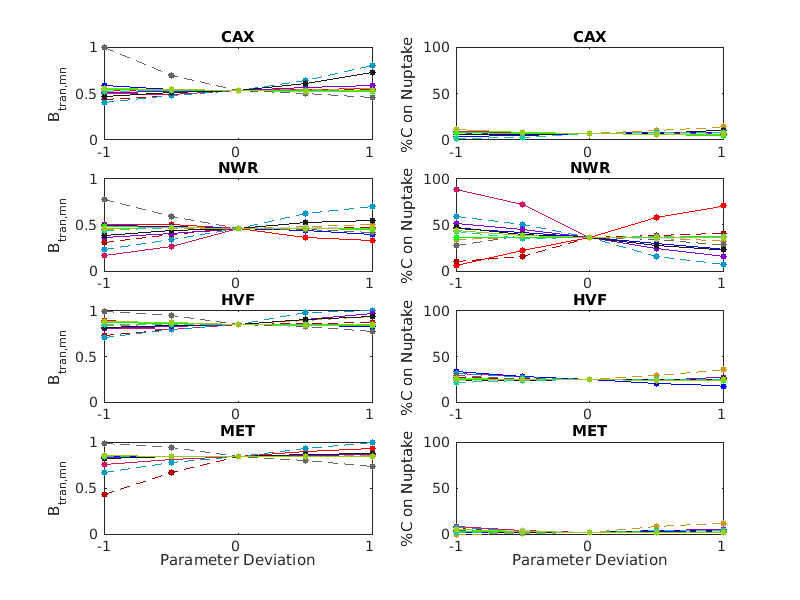
\includegraphics[width=0.5\textwidth, right]{lion-lo9
     \includegraphics[width=1.3\textwidth, left]{matlab/figures/btran_npp.png}
     \caption{Response of drought index ($B_{tran,mn}$ and the \% of NPP spent on Nitrogen uptake to parameter perturbation across -1 to +1 range of parameter variation at the Caxiuan\~a (CAX), Niwot Ridge (NWR), Harvard Forest (HVF) and Metolious MET) sites.}
     \label{btran state}
 \end{figure}
 
 \begin{figure}[h]
    % \centering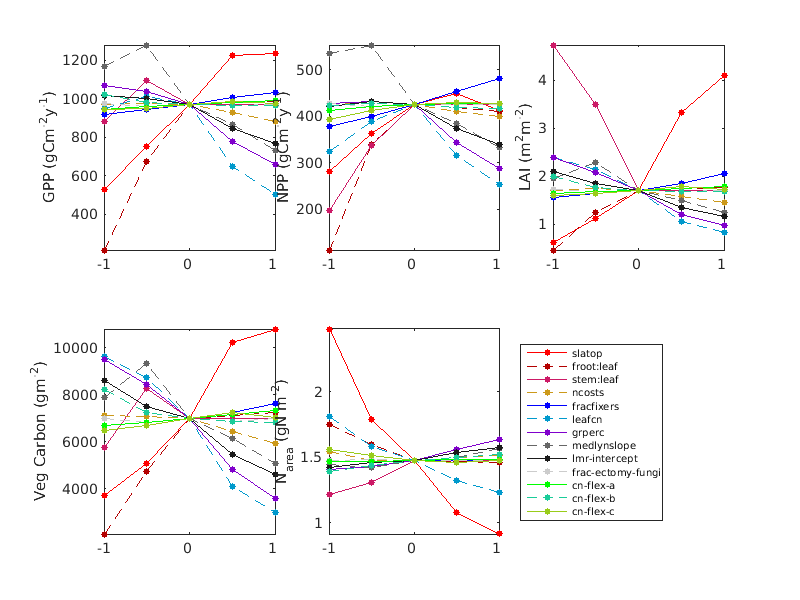
\includegraphics[width=0.5\textwidth, right]{lion-lo9
     \includegraphics[width=1.3\textwidth, left]{matlab/figures/NOVc_STATE_1CLM50defpft_trans_1x1pt_US-NR1_ens_MIC_y1_2012.png}
     \caption{Response of control model states and fluxes to parameter perturbation across -1 to +1 range of parameter variation at Niwot Ridge.}
     \label{NR1 state}
 \end{figure}
 
  \begin{figure}[h]
    % \centering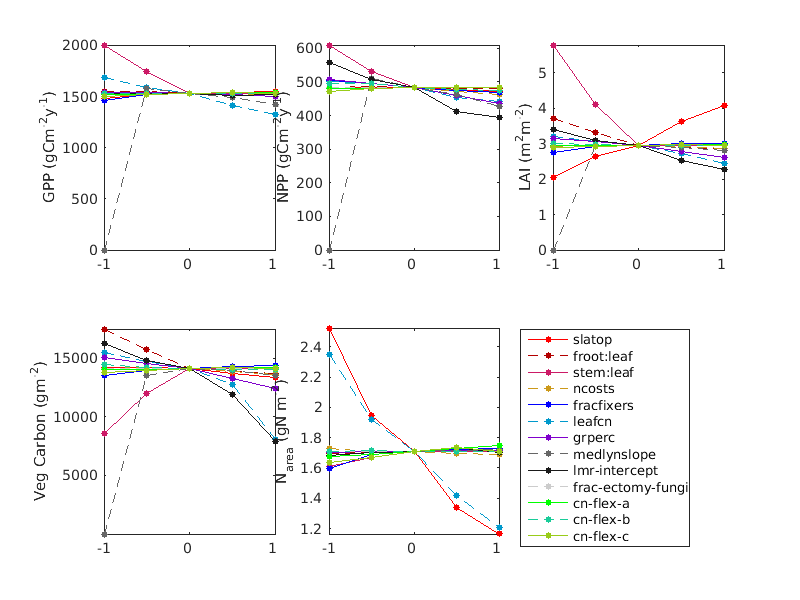
\includegraphics[width=0.5\textwidth, right]{lion-lo9
     \includegraphics[width=1.3\textwidth, left]{matlab/figures/NOVc_STATE_1CLM50defpft_trans_1x1pt_Br-cax_ens_MIC_y1_2012.png}
     \caption{Response of control model states and fluxes to parameter perturbation across -1 to +1 range of parameter variation at Caxiuan\~a National Forest}
     \label{CAX state}
  \end{figure}
  
 \begin{figure}[h]
    % \centering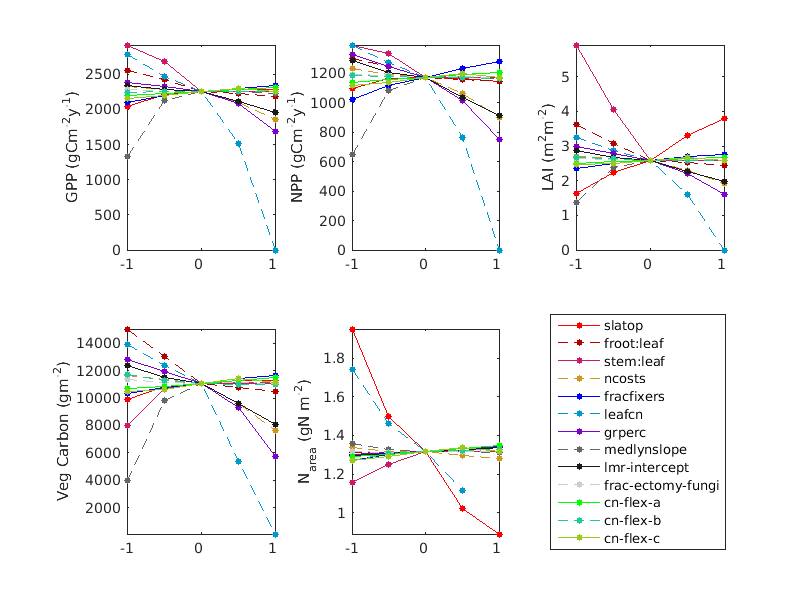
\includegraphics[width=0.5\textwidth, right]{lion-lo9
     \includegraphics[width=1.3\textwidth, left]{matlab/figures/NOVc_STATE_1CLM50defpft_trans_1x1pt_US_Ha1_ens_MIC_y1_2012.png}
     \caption{Response of control model states and fluxes to parameter perturbation across -1 to +1 range of parameter variation at Harvard Forest}
     \label{HVF state}
 \end{figure} 
  
 \begin{figure}[h]
    % \centering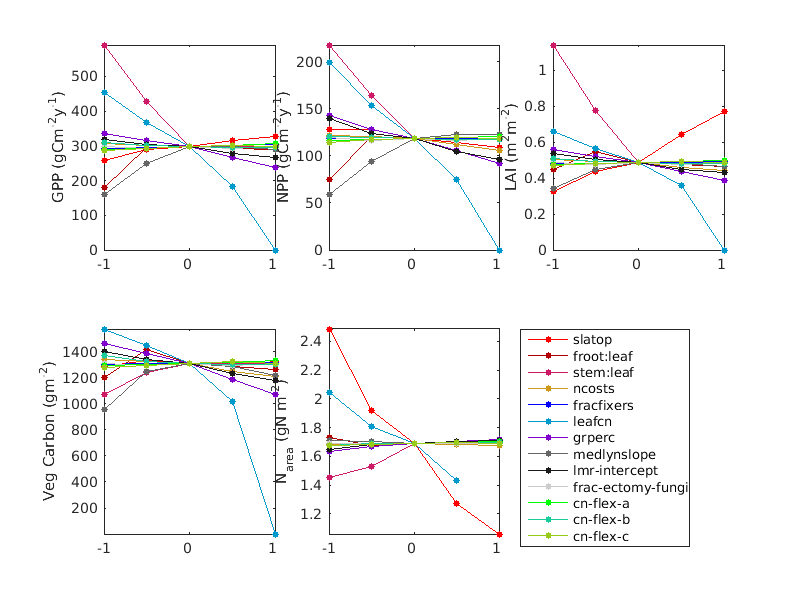
\includegraphics[width=0.5\textwidth, right]{lion-lo9
     \includegraphics[width=1.3\textwidth, left]{matlab/figures/NOVc_STATE_1CLM50defpft_trans_1x1pt_US-Me2_ens_MIC_y1.png}
     \caption{Response of control model states and fluxes to parameter perturbation across -1 to +1 range of parameter variation at Metolius Forest}
     \label{MET state}
 \end{figure}


  \begin{figure}[h]
    % \centering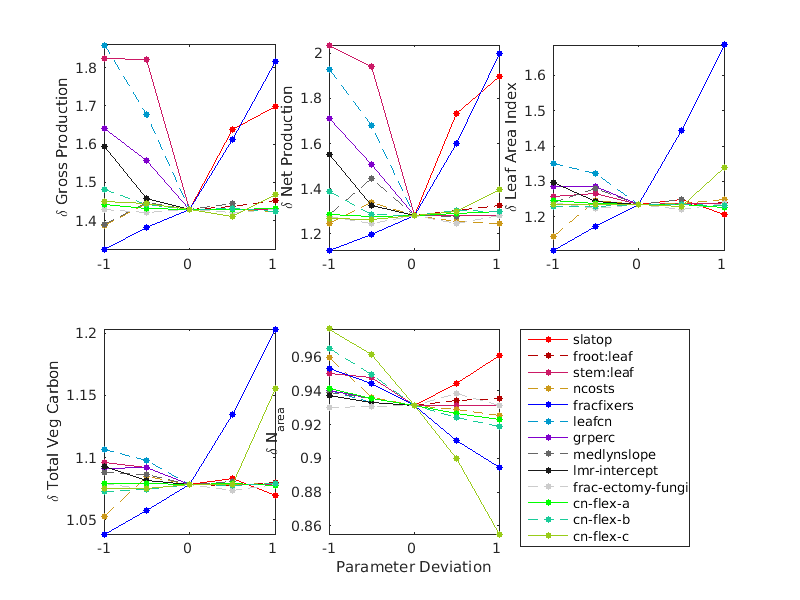
\includegraphics[width=0.5\textwidth, right]{lion-lo9
     \includegraphics[width=1.3\textwidth, left]{matlab/figures/NOVc_FERT_1CLM50defpft_celev_1x1pt_US-NR1_ens_MIC_p1_2012.png}
     \caption{Influence of parametric variation (over the range tested: -1 to +1) on the influence of 15 years of CO$_{2}$ fertilization (550ppm) at Niwot Ridge}
     \label{NR1 celev}
  \end{figure}
  
  \begin{figure}[h]
    % \centering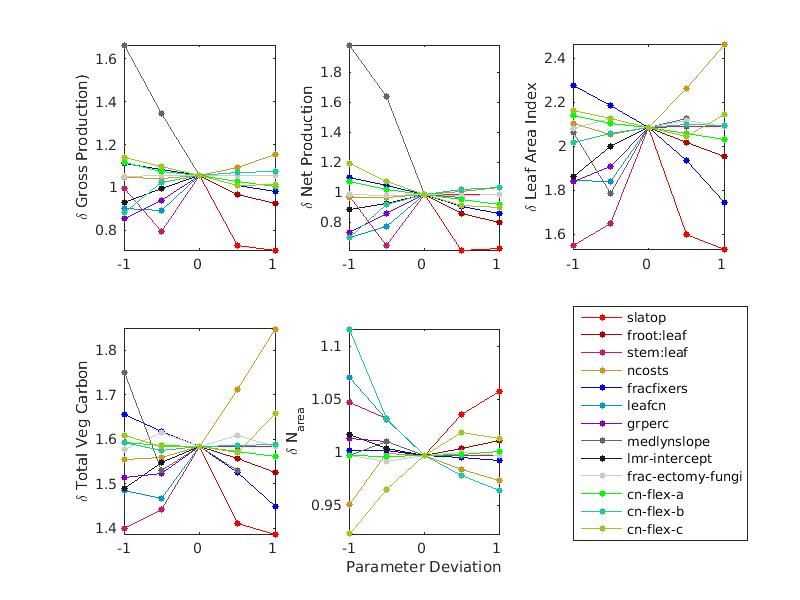
\includegraphics[width=0.5\textwidth, right]{lion-lo9
     \includegraphics[width=1.3\textwidth, left]{matlab/figures/NOVc_FERT_1CLM50defpft_ndep_1x1pt_US-NR1_ens_MIC_p1.png}
     \caption{Influence of parametric variation (over the range tested: -1 to +1) on the influence of 15 years of Nitrogen fertilization (+5 kgN m$^{2}$ y$^{-1}$) at Niwot Ridge}
     \label{NR1 ndep}
 \end{figure}
      
 \begin{figure}[h]
     \centering
     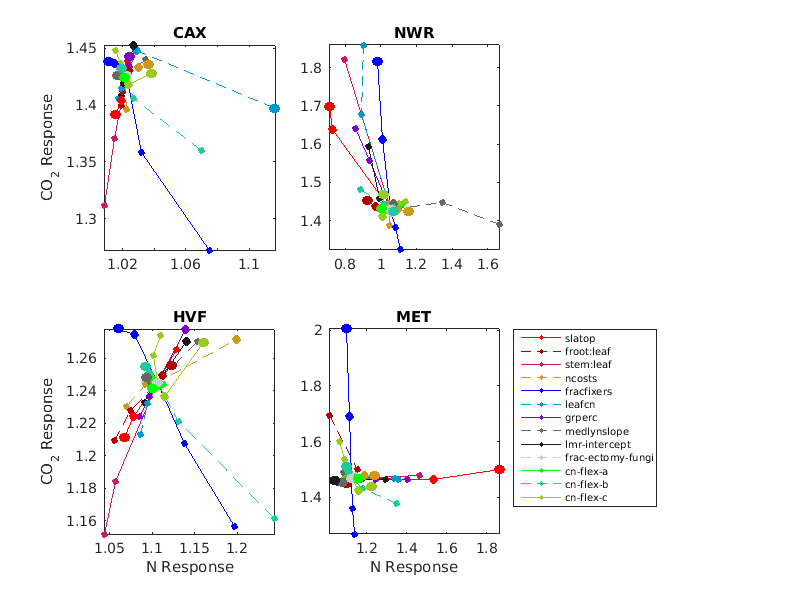
\includegraphics[width=1.55\textwidth, left]{matlab/figures/NOVc_CNdep_GPP1__p2012.png}
     \caption{Influence of parametric variation on the impact of 15 years of CO$_{2}$ and N fertilization on gross primary productivity (GPP), across the Caxiuan\~a (CAX), Niwot Ridge (NWR), Harvard Forest (HVF) and Metolious MET) sites. }
     \label{GPP CO2 and N respones 2001}
  \end{figure}
  
 \begin{figure}[h]
     \centering
     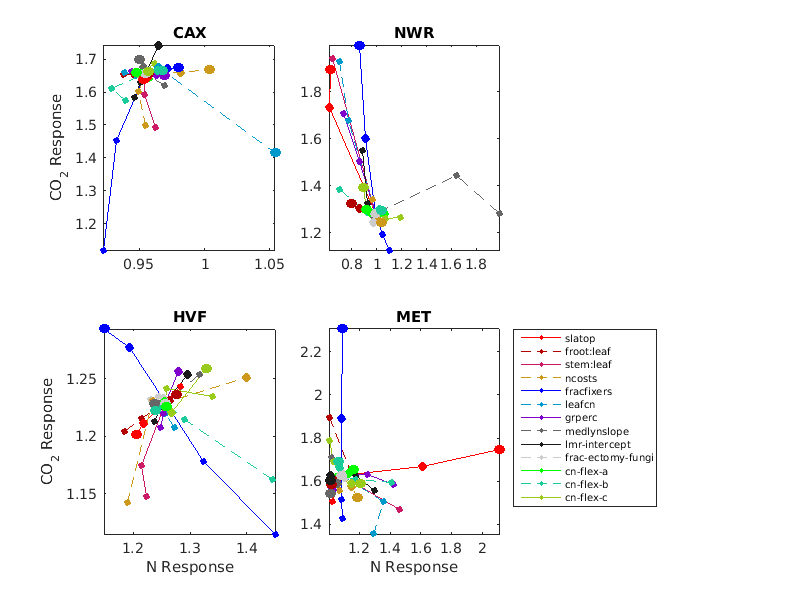
\includegraphics[width=1.55\textwidth, left]{matlab/figures/NOVc_CNdep_NPP1__p2012.png}
     \caption{Influence of parametric variation on the impact of 15 years of CO$_{2}$ and N fertilization on net primary productivity (NPP), across the Caxiuan\~a (CAX), Niwot Ridge (NWR), Harvard Forest (HVF) and Metolious MET) sites.}
     \label{NPP CO2 and N respones 2001}
  \end{figure}
  
  \begin{figure}[h]
     \centering
     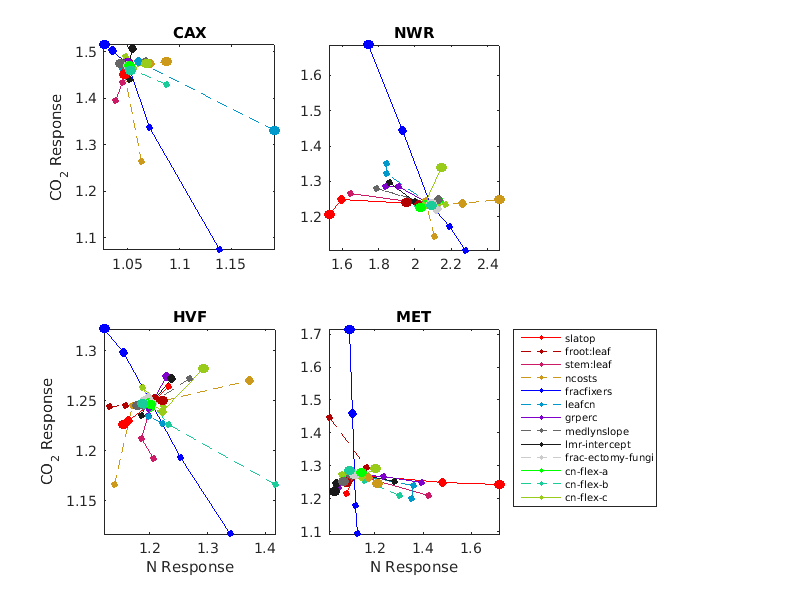
\includegraphics[width=1.55\textwidth, left]{matlab/figures/NOVc_CNdep_TLAI1__p2012.png}
     \caption{Influence of parametric variation on the impact of 15 years of CO$_{2}$ and N fertilization on leaf area index (LAI), across the Caxiuan\~a (CAX), Niwot Ridge (NWR), Harvard Forest (HVF) and Metolious MET) sites.}
     \label{LAI CO2 and N respones 2001}
  \end{figure}
  


\section{To Do}
Maybe include the delta in N expenditure. 

Site details


\end{document}

